% begin module optimization-ex1
\begin{frame}
\begin{example}
\alert<handout:0| 10>{A farmer has 2400 ft of fencing} and wants to fence off a rectangular field that borders a straight river.  He doesn't need to put fencing along the river.  What are the dimensions of the field with the largest area?
\begin{columns}[c]
\column{.5\textwidth}
\psset{xunit=0.7cm, yunit=0.7cm}
\begin{pspicture}(-3.1,-2.1)(3.1,2.7)
\psframe*[linecolor=white](-3.1,-2.1)(3.1,2.7) 
\psdot[linecolor=red!1](0, 2.6)
\tiny
%Function formula: 1/20 (\sin{}(x)) 
\psplot[linecolor=blue, plotpoints=1000]{-3}{3}{x 57.29578 mul sin 0.05 mul } 
%Function formula: -1+1/20 (\sin{}(2+6/5*(x))) 
\psplot[linecolor=blue, plotpoints=1000]{-3}{3}{x 1.2 mul 2 add 57.29578 mul sin 0.05 mul -1 add }
\uncover<handout:0|2>{
\psline[linecolor=red](-2, 0)(-2, 0.4)(2, 0.4)(2, 0)
\rput[r] (-2.2, 0.2){$200$}
\rput[l] (2.2, 0.2){$200$}
\rput[b] (0, 0.6){$2000$}
} 
\uncover<handout:0|3>{
\psline[linecolor=red](-1.8, 0)(-1.8, 0.6)(1.8, 0.6)(1.8, 0)
\rput[r] (-2, 0.3){$300$}
\rput[l] (2, 0.3){$300$}
\rput[b] (0, 0.8){$1800$}
} 
\uncover<handout:0|4>{
\psline[linecolor=red](-1.4, 0)(-1.4, 1)(1.4, 1)(1.4, 0)
\rput[r] (-1.6, 0.5){$500$}
\rput[l] (1.6, 0.5){$500$}
\rput[b] (0, 1.2){$1400$}
} 
\uncover<5>{
\psline[linecolor=red](-1.2, 0)(-1.2, 1.2)(1.2, 1.2)(1.2, 0)
\rput[r] (-1.4, 0.6){$600$}
\rput[l] (1.4, 0.6){$600$}
\rput[b] (0, 1.4){$1200$}
} 
\uncover<handout:0|6>{
\psline[linecolor=red](-0.8, 0)(-0.8, 1.6)(0.8, 1.6)(0.8, 0)
\rput[r] (-1, 0.8){$800$}
\rput[l] (1, 0.8){$800$}
\rput[b] (0, 1.8){$800$}
} 
\uncover<handout:0|7>{
\psline[linecolor=red](-0.6, 0)(-0.6, 1.8)(0.6, 1.8)(0.6, 0)
\rput[r] (-0.8, 0.9){$900$}
\rput[l] (0.8, 0.9){$900$}
\rput[b] (0, 2){$600$}
} 
\uncover<handout:0|8>{
\psline[linecolor=red](-0.2, 0)(-0.2, 2.2)(0.2, 2.2)(0.2, 0)
\rput[r] (-0.4, 1.1){$1100$}
\rput[l] (0.4, 1.1){$1100$}
\rput[b] (0, 2.4){$200$}
} 
\uncover<handout:0|9->{
\psline[linecolor=red](-1.4, 0)(-1.4, 1)(1.4, 1)(1.4, 0)
\rput[r] (-1.6, 0.5){$x$}
\rput[l] (1.6, 0.5){$x$}
\rput[b] (0, 1.2){$y$}
} 
\end{pspicture}
%\ \only<handout:0| -2>{%
%\uncover<2>{%
%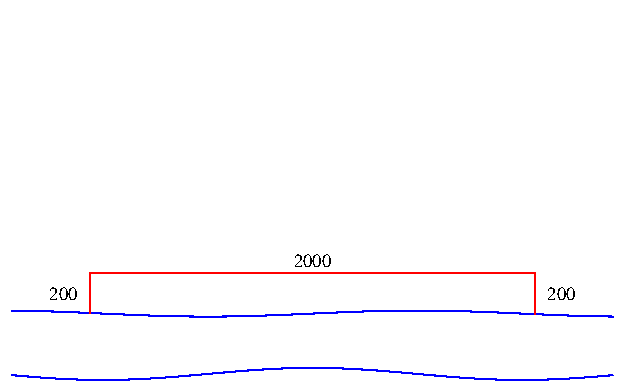
\includegraphics[width=5cm]{optimization/pictures/04-07-ex1a.pdf}%
%}}%
%\only<handout:0| 3>{%
%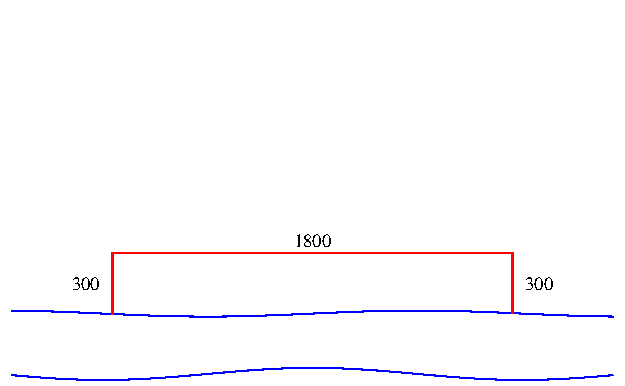
\includegraphics[width=5cm]{optimization/pictures/04-07-ex1b.pdf}%
%}%
%\only<handout:0| 4>{%
%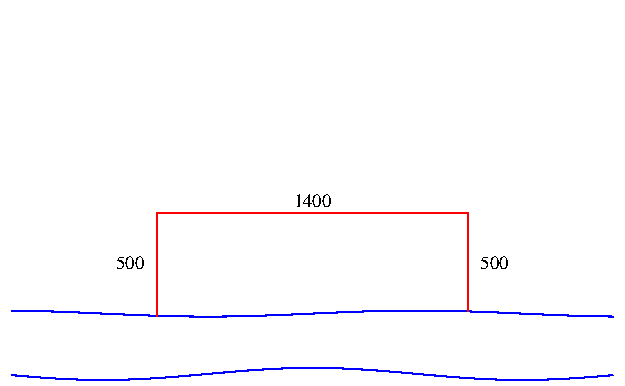
\includegraphics[width=5cm]{optimization/pictures/04-07-ex1c.pdf}%
%}%
%\only<handout:0| 5>{%
%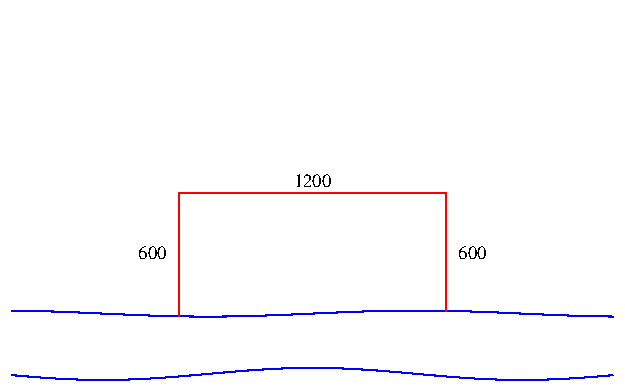
\includegraphics[width=5cm]{optimization/pictures/04-07-ex1d.pdf}%
%}%
%\only<handout:0| 6>{%
%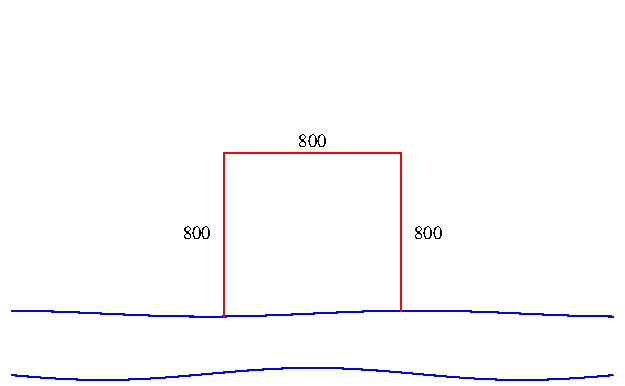
\includegraphics[width=5cm]{optimization/pictures/04-07-ex1e.pdf}%
%}%
%\only<handout:0| 7>{%
%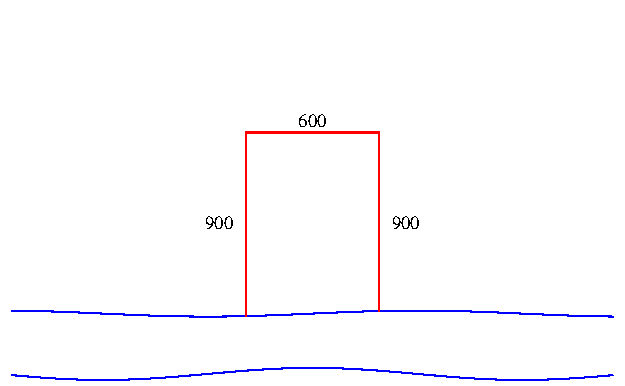
\includegraphics[width=5cm]{optimization/pictures/04-07-ex1f.pdf}%
%}%
%\only<handout:0| 8>{%
%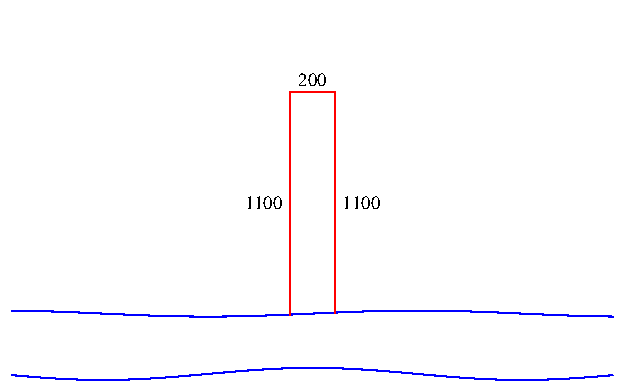
\includegraphics[width=5cm]{optimization/pictures/04-07-ex1g.pdf}%
%}%
%\only<9->{%
%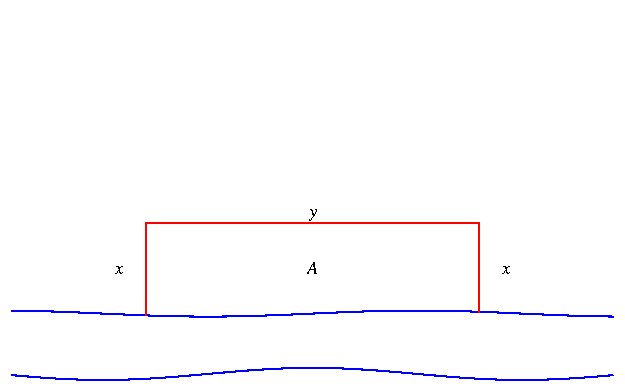
\includegraphics[width=5cm]{optimization/pictures/04-07-ex1h.pdf}%
%}%

\uncover<2->{%
Area $ = %
\only<9->{%
A = xy
}%
\only<handout:0| -8>{%
\only<handout:0| -2>{200}%
\only<handout:0| 3>{300}%
\only<handout:0| 4>{500}%
\only<handout:0| 5>{600}%
\only<handout:0| 6>{800}%
\only<handout:0| 7>{900}%
\only<handout:0| 8>{1100}%
\cdot%
 \only<handout:0| -2>{2000} %
\only<handout:0| 3>{1800}%
\only<handout:0| 4>{1400}%
\only<handout:0| 5>{1200}%
\only<handout:0| 6>{800}%
\only<handout:0| 7>{600}%
\only<handout:0| 8>{200}%
= %
\only<handout:0| -2>{400,000}%
\only<handout:0| 3,7>{540,000}%
\only<handout:0| 4>{700,000}%
\only<handout:0| 5>{720,000}%
\only<handout:0| 6>{640,000}%
\only<handout:0| 8>{220,000}%
}$\only<handout:0| -8>{ft$^2$}
}%
\uncover<20->{%
\abovedisplayskip=0pt
\belowdisplayskip=0pt
\[
\begin{array}{r|r}
x & A(x)\\
\hline
\alert<handout:0| 21-22>{0} & \alert<handout:0| 22>{\uncover<22->{0}}\\
\alert<handout:0| 23-24,27>{600} & \alert<handout:0| 24,27>{\uncover<24->{720,000}}\\
\alert<handout:0| 25-26>{1200} & \uncover<26->{\alert<handout:0| 26>{0}}
\end{array}
\]
}%
\column{.5\textwidth}
\uncover<9->{%
Let $x$ and $y$ denote the depth and width of the rectangle (in feet).  Let $A$ be its area.%
}%
\abovedisplayskip=0pt
\belowdisplayskip=0pt
\abovedisplayshortskip=0pt
\belowdisplayshortskip=0pt
\begin{align*}
\uncover<10->{2x + y} & \uncover<10->{=}  \uncover<10->{2400}\\
\uncover<11->{\alert<handout:0| 13>{y}} & \uncover<11->{\alert<handout:0| 13>{=}}  \uncover<11->{\alert<handout:0| 13>{2400 - 2x}}\\
\uncover<12->{A} & \uncover<12->{=}  \uncover<12->{x\alert<handout:0| 13>{y}} \uncover<13->{=  x(\alert<handout:0| 13>{2400-2x})}\\
& \uncover<14->{=}  \uncover<14->{2400x - 2x^2}%
\end{align*}
\uncover<15->{Notice that $0\leq x \leq 1200$.}

\uncover<16->{%
Maximize the function $A(x)$:
\[
\alert<handout:0| 16-17>{A'(x) = \uncover<17->{2400 - 4x}}%
\]
}%
\uncover<18->{%
Critical number: \alert<handout:0| 18-19>{$x = $ \uncover<19->{$600$.}} 
}%
\end{columns}
\uncover<27->{%
Therefore the maximum area occurs when $x = 600$ft and $y = 1200$ft.
}%
\end{example}
\end{frame}
% end module optimization-ex1